\section{Codebase}\label{sec:code}
As a baseline we used the libDAI library \cite{Mooij_libDAI_10} which provides an implementation for LBP using the maximal residual updating scheme. With the library, it was simple to implement the recommendation system as proposed in  \cite{Ha:2012:TRT:2396761.2398636}.

\mypar{Code structure}
Figure \ref{overviewflow} shows a high-level overview of the code structure. After an initialization phase the BP algorithm is invoked which loops until a specified maximum number of iterations is reached, the maximum residual becomes zero or the change in the updated messages is smaller than the specified tolerance. In every iteration, \texttt{findMaxResidual} is called to determine the message that should be updated next by \texttt{updateMessage}. The actual update step is simple, because it only assigns \texttt{new\-Message} to message. The costly part of the algorithm is the re-computation of \texttt{newMessage} for all neighbouring nodes that are affected by the change. To do so, \texttt{calcNew\-Message} is called for every candidate, which first computes a product over all incoming messages (see \texttt{calc\-IncomingMessageProduct}) and then marginalizes this product of messages over all other variables (\texttt{margina\-lizeProductOntoMessage}). 

%\lstset{basicstyle=\tiny\ttfamily}
%\begin{table}
%\begin{lstlisting}
%init()
%while (not done)
%   messageToUpdate <-- findMaxResidual;
%\end{lstlisting}
%\caption{Pseudo code for Residual BP}
%\end{table}

The methods that get called the most often are \texttt{update\-Residual}, \texttt{calcIncomingMessageProduct} and \linebreak\texttt{marginalizeProductMessage}. Hence, the optimizations will mostly focus on these.

\begin{figure}\centering
    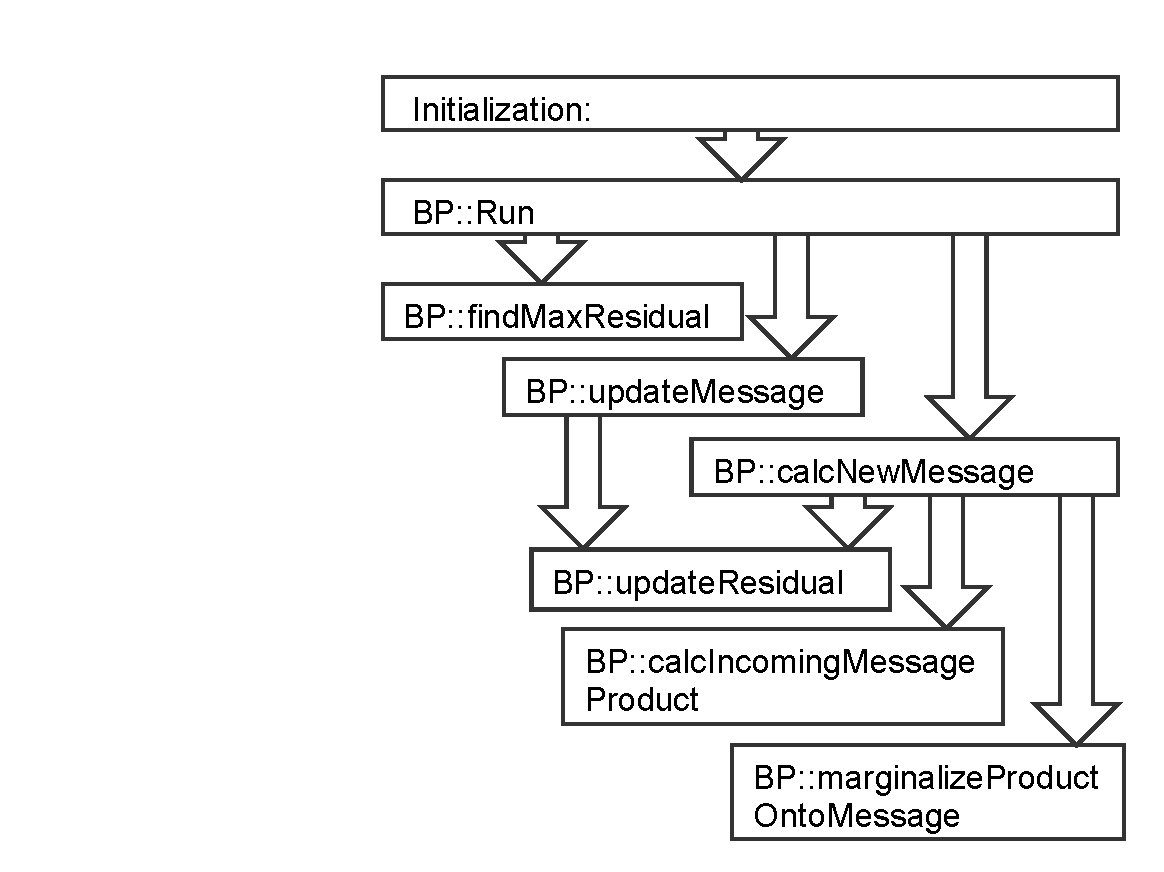
\includegraphics[scale=0.5, trim={6.45cm 0cm 0 1.25cm},clip]{graphics/loopybp-compact.pdf}
  \caption{Flow (top to bottom) of our program. Arrows denote that a methods gets called from an other, BP is the namespace used for all functions that deal with belief propagation.\label{overviewflow}}
\end{figure}

